\documentclass[12pt,a4paper]{article}
\usepackage[top=25.4mm, bottom=25.4mm, left=19.1mm, right=19.1mm]{geometry}


\usepackage[latin2]{inputenc}
\usepackage{graphicx}
\graphicspath{ {./images/} }
\usepackage{ulem}
\usepackage{amsmath}
\usepackage[document]{ragged2e}

\setlength{\parindent}{4em}
\setlength{\parskip}{1em}
\usepackage{hyperref}

\usepackage{fancyhdr}
\pagestyle{fancy}
\fancyhf{}
\fancyhead[LO]{\textbf{\small IoT and Smart Analytics}\\
\text{\small A Program by IIITH and TalentSprint}}

\usepackage{xcolor}
\usepackage{lipsum}

\rhead{\begin{picture}(0,0) \put(-250,-2){
\includegraphics[width=9cm]{EXP_08_Images/ts-iisc-logo-pr.png}} \end{picture}}
\cfoot{\thepage}


\begin{document}

\begin{center}

\textbf{\large \\EXPERIMENT 15 }\\[6pt]
\text{Sleep Mode with Interrupt, Sleep Mode with Watchdog (WDT), and External Interrupt in Arduino }
\end{center}

\textbf{\large LEARNING OBJECTIVES:}\\[3pt]
At the end of this experiment, participants will be able to:\vspace{-6mm}\begin{enumerate}
 \setlength\itemsep{-0.3em}
\item Understand \& use Sleep Mode with Interrupt in Arduino\\
\item Understand \& use Sleep Mode with Watchdog in Arduino\\ 
\item Understand \& use External Interrupts in Arduino
\end{enumerate}
\textbf{\large APPARATUS REQUIRED:}\\
\vspace{-3mm}
\begin{enumerate}
 \setlength\itemsep{-0.3em}
\item Arduino Module-1pcs \\
\item Breadboard-1pcs\\
\item USB cable-1pcs\\
\item LED-1pcs\\
\item Push button -1pcs\\
\item Buzzer-1pcs\\
\item Resistor-2pcs\\
\item Jumper wires\\
\end{enumerate}

\begin{justify}
\textbf{\large PROCEDURE}\\[3pt]
\textbf{A)	Sleep Mode with Interrupt }\\[3pt]
\textbf{Hardware and software setup :} The fig. 1 below shows the circuit diagram for the experiment. Built-in LED connected to pin 13 used here and after blinking for 5 times the Arduino goes to sleep mode. Once pin 2 is triggered through the push button it wakes up again. Code is written with explanations in comments.\end{justify}


\begin{center} 
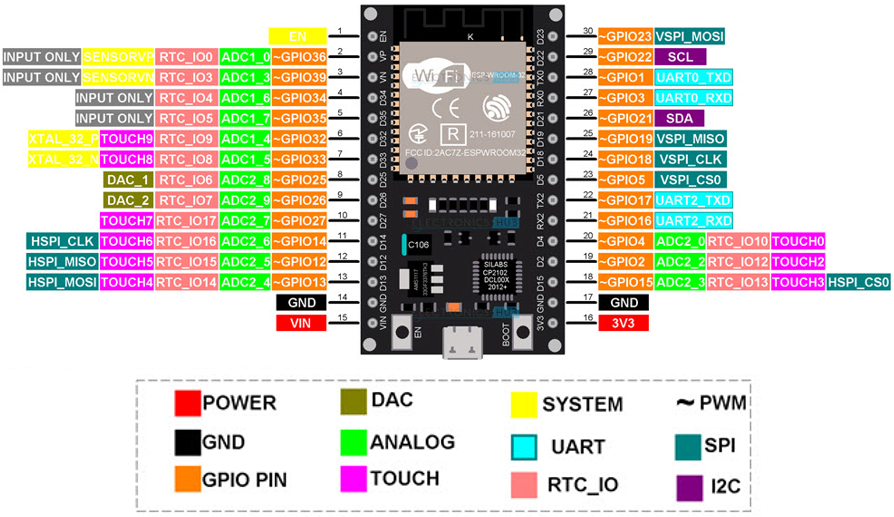
\includegraphics[scale=0.7]{EXP_15_Images/fig1.PNG}
\end{center}
\begin{center} {Figure 1. Circuit diagram for sleep with interrupt}\end{center}

\hspace{1.5cm}\textbf{\large Code:}\\[6pt]
\setlength{\parindent}{8eM}

\textcolor{blue}{/* 5 different modes are:  SLEEP\_MODE\_IDLE , SLEEP\_MODE\_ADC\\
 *  SLEEP\_MODE\_PWR\_SAVE, SLEEP\_MODE\_STANDBY\\
 *  SLEEP\_MODE\_PWR\_DOWN $\rightarrow$ arguments\\ used to set the sleep mode in function set\_sleep\_mode()*/}\\
\#include$<$avr/sleep.h$>$\\
int led=13; \textcolor{blue}{// LED connected}\\
 int count=0;\textcolor{blue}{ //variable to control how many times LED blinks before sleep}\\[14pt]

 void setup()\\
 \{\\
  sleep\_enable(); \textcolor{blue}{ // enabling the sleep capability}\\
  set\_sleep\_mode(SLEEP\_MODE\_PWR\_DOWN);  \textcolor{blue}{// the type of sleep mode.\\ Default is Idle}\\
  pinMode(led,OUTPUT); \textcolor{blue}{// setup the LED pin to output}\\
 \}\\[14pt]

 void loop()\\
 \{\\
  if (count$<$5)\\
    \{\\
      digitalWrite(led,HIGH);\\
      delay(1000);\\
      digitalWrite(led,LOW);\\
      delay(1000);\\
      count++;\\
      \}\\
    else\\
     \{\\
\textcolor{blue}{//After blinking LED, sets up interrupt & go to sleep\\
      //Note sleep will happens only once since it is disabled in ISR}\\
      attachInterrupt(0,interruptFunction,HIGH);\\
      sleep\_cpu(); \textcolor{blue}{// enter in sleep mode. Next code that will be executed is ISR \\
      when interruptswakes the Arduino from sleep}\\
      count=0;\\
    \} \\      
 \}\\[14pt]
 
void interruptFunction()\\
    \{\\
      detachInterrupt(0); \textcolor{blue}{// this function turns the interrupt off}\\
      sleep\_disable(); \textcolor{blue}{ // disable the sleep mode so even if call to execute the sleep,\\it will be ignored now.  \\Try by commenting this line, observe the result}\\
      \}

\vspace{20mm}



\setlength{\parindent}{0pt}
\begin{justify}
\textbf{B) Sleep Mode with Watchdog (WDT)}\\[3pt]
{\textbf{Hardware and software setup :}Built-in LED is used. Code is explained with comments. Note the Arduino goes to sleep mode for 8 seconds after every three blinks of LED .The sleep for 8 seconds is being counted by WDT and it restarts after that time.\end{justify}

\hspace{1.5cm}\textbf{\large Code:}\\[6pt]
\setlength{\parindent}{8eM}

\#include $<$avr/sleep.h$>$\\
 #include$<$avr/wdt.h$>$\\
 int led=13;\\
 int tog=1;\\[14pt]

 void setup()\\
  \{\\
    wdt\_disable(); \textcolor{blue}{//recommended}\\
    pinMode(led,OUTPUT); \textcolor{blue}{//set up the LED pin to output}\\
  \}\\[14pt]

void loop()\\
  \{\\
    if(tog)\\
        \{ \\
          digitalWrite(led,HIGH);\\
          delay(1000);\\
          digitalWrite(led,LOW);\\
          delay(1000);\\
          digitalWrite(led,HIGH);\\
          delay(1000);\\
          digitalWrite(led,LOW);\\
          delay(1000);\\
          tog=0;\\
        \}\\
     else\\
        \{\\
          digitalWrite(led,HIGH);\\
          delay(1000);\\
          digitalWrite(led,LOW);\\
          \textcolor{blue}{// function that we are going to define using WDT, takes byte argument}\\
          delayWDT(0b00100001); \textcolor{blue}{//8S:WDP3=1 & WDP0=1//4S: WDP3=1& WDP0=0}\\
          tog=1;\\
          \} \\
    \}
    \vspace{30mm}

\textcolor{blue}{/*function below serves as a power-saving delay fun.Argument is byte type.\\
 * for setting a delay time. The function sets up sleep in a power down state.\\
 * The function then sets up the WDT timer in interrupt mode and sets it.\\
 * Then, it puts the Arduino to sleep for the set time,upon wake up the \\WDT & sleep mode are shut off.*/}\\[9pt]
void delayWDT(byte timer)\\
 \{\\
  sleep\_enable(); \textcolor{blue}{// enable the sleep capability}\\
  set\_sleep\_mode(SLEEP\_MODE\_PWR\_DOWN); \textcolor{blue}{//set type of sleep mode}\\
  
  ADCSRA \& = $\sim$ (1$<<$ ADEN);\textcolor{blue}{ // Turn off ADC before going to sleep}
  
  WDTCSR $|$ =(1 $<<$WDCE) $|$ (1 $<<$ WDE); \textcolor{blue}{ //set the WDCE\& WDE bit\\and  clear when set the prescaler \& WDIF }
  
  WDTCSR=(1$<<$WDIE) $|$ timer;\textcolor{blue}{ //(1$<<$WDIE) : enabling interrupt mode}\\
  wdt\_reset();\textcolor{blue}{ //Reset the WDT so that timer start from zero position}\\
  
  sleep\_cpu(); \textcolor{blue}{//enter sleep mode, watchdog timer running in background.\\
  //Next code that will be executed is the ISR when}\\
  sleep\_disable(); \textcolor{blue}{//disable sleep mode}\\
  ADCSRA $|$ =(1$<<$ADEN); \textcolor{blue}{//Turn the ADC back on}\\
  \}\\[14pt]
  
\textcolor{blue}{//This is the interrupt service routine for the WDT\\//It is called when the WDT times out}\\

  ISR(WDT\_vect)\\
  \{\\
    wdt\_disable();\\
    MCUSR=0; \textcolor{blue}{// Clear WDT flage since it is disabled}\\ 
    \}\\



\setlength{\parindent}{0pt}
\begin{justify}
\textbf{C)	External Interrupt}\\[3pt]
{\textbf{Hardware and software setup :}In this experiment, we are going to implement the external interrupt. We will detect if a circuit is complete or broken. As soon as the circuit breaks, we will trigger the alarm using an interrupt service routine (ISR). The LED and buzzer will turn on as the alarm. This type of circuit finds use in emergency systems, burglar alarm systems, etc. Connection diagram is given below.\end{justify}

\begin{center} 
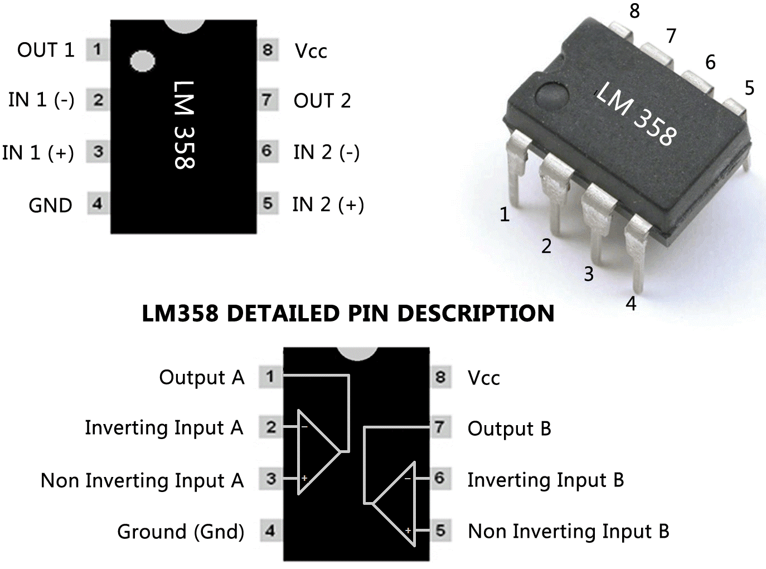
\includegraphics[scale=0.7]{EXP_15_Images/fig2.PNG}
\end{center}
\begin{center} {Figure 2.Circuit diagram for external interrupts}\end{center}


\hspace{1.5cm}\textbf{\large Code:}\\[6pt]
\setlength{\parindent}{8eM}


const byte ledPin = 7;\\
const byte interruptPin = 3;\\
volatile int state = LOW;\\
\textcolor{blue}{// volatile keyword helps to prevent compiler optimization and\\
//variable value is always fetched from the main memory}\\[14pt]

void setup()\\
\{\\
  pinMode(ledPin, OUTPUT);\\
  pinMode(interruptPin,INPUT);\\
  attachInterrupt(digitalPinToInterrupt(interruptPin), alarm,FALLING);\\
  \textcolor{blue}{// FALLING keyword triggers the interrupt on the falling edge i.e\\
//HIGH to LOW state change of the pin}\\
\}\\[14pt]

void loop()\\
\{\\
  digitalWrite(ledPin, state);\\
\}\\[14pt]
void alarm()\\
\{\\
  state^=1;\\
\}\\





\vspace{30mm}

\setlength{\parindent}{0eM}
\begin{justify}
\begin{center} \textbf{\large CONCEPT DRILLS: BARE METAL PROGRAMMING }\end{center}
\vspace{-3mm}
\begin{enumerate}
 \setlength\itemsep{-0.3em}
\item Using Timer 1 with a prescaler value of 256, blink an LED connected to the 7th pin of Port D. Show the relevant calculation.
\item Use Timer 1 with a prescaler value of 256. Blink an LED connected to the 7th pin of Port D by making a user-defined delay function using the timer flag concept. Show the relevant calculation.

\end{enumerate}
\end{justify}
\end{document}